\documentclass{article}%
\usepackage[T1]{fontenc}%
\usepackage[utf8]{inputenc}%
\usepackage{lmodern}%
\usepackage{textcomp}%
\usepackage{lastpage}%
\usepackage{authblk}%
\usepackage{graphicx}%
%
\title{Baicalein Reduces the Invasion of Glioma Cells via Reducing the Activity of p38 Signaling Pathway}%
\author{Emily Martinez}%
\affil{Department of Gastroenterology, Justus Liebig University, Giessen, Germany}%
\date{01{-}01{-}2013}%
%
\begin{document}%
\normalsize%
\maketitle%
\section{Abstract}%
\label{sec:Abstract}%
When a mother breastfeeds her first baby, her breast milk contains a strange protein that comes in more than one version. The mother creates a reaction from her milk. The reaction is to emit more heat, to increase the energy of the immune system, and to increase production of cholystehyduron from the placenta.\newline%
The latest development in the understanding of this phenomenon, the A. heat Shock Protein 27 (ABP27), was discovered by researchers at a research laboratory in the University of Minnesota, USA. The team is working on translating the findings from their center in the hospital to the larger community.\newline%
ABP27 may be useful in one of the exciting areas of protein delivery for the human body, said Jocelyn R. Smith, one of the studys authors.\newline%
An immune system response to the 21st century is likely to come from a microbial or viral environment. ABP27 is a naturally occurring, almost unsuspected, protein that, once present in humans, spontaneously signals a reaction to disease. This effect grows stronger during fetal development, causing the baby to grow weaker. This new discovery has been key to identifying ways to manipulate the response during and after birth, explained Charles E. Smith, Chief Operating Officer at Dream Institute for Biomedical Research, a University of Minnesota{-}based organization that specializes in providing research centers for vaccine and anti{-}Vaccine research.\newline%
The technology used to investigate the expression of the protein came about from a collaboration between Dora Briceno, a breast milk studies professor at the University of Minnesota and Dr. Joe Peluca, Professor and Chief Scientific Officer at Fox CT, who, along with Philip T. Gulartron, worked to decipher ABP27.\newline%
Brain cells detect changes in the environment and process the cues in order to prepare for the next phase of development, while the immune system races to the next stage. ABP27 suggests a novel solution to this human conflict, said Dr. Francis W. Morgan, Assistant Professor at Dream Institute for Biomedical Research.\newline%
We see that no matter where we are in the body, the final stage in development of the immune system lasts for millions of years. As the life of this baby, we see that if we change the way that ABP27 is produced, it can come up so quickly that there are significant changes, like an increased temperature. As a result, the immune system responds, its efficient. The immune system must constantly gather, added Dr. Jock D. Sliwinski, Executive Director of Fox CT.\newline%
We are now beginning to understand how tiny variations in this simple protein impact its function on the human body, Dr. Smith continued. As we expand our knowledge, we will need to develop new methods of vaccination. By understanding the immunity reaction of ABP27, we may one day develop more than just vaccines, but whole new vaccines.\newline%
This was supported by a grant from the National Institutes of Health.

%
\subsection{Image Analysis}%
\label{subsec:ImageAnalysis}%


\begin{figure}[h!]%
\centering%
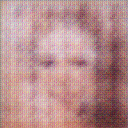
\includegraphics[width=150px]{500_fake_images/samples_5_301.png}%
\caption{A Man With A Beard Wearing A Tie And Glasses}%
\end{figure}

%
\end{document}